\chapter{Determination of \lambdaWZ through VBS WH production}
\begin{aquote}{Peter Higgs, Edinburgh University press conference, 2012}
    It's very nice to be right sometimes.
\end{aquote}
% In this chapter, a simple, yet powerful insight is derived from the statistical analysis of proton-proton data collected by the CMS Experiment. 
% This analysis serves as a blueprint for the following chapter, in which a more involved, but thematically similar, analysis is documented. 
% Moreover, its structure reveals how CMS data is used to make statements about the Standard Model in general. 
% First, a ``signal'' process is defined, motivated by some exciting new theory or by the simple fact that it has never been considered before. 
% However, the signal process is often incredibly rare compared to the sheer amount of uninteresting junk (``background'' processes) produced at the LHC. 
% The signal is therefore carefully studied for features that distinguish it from the background. 
% Most likely, some background processes have similar, or even identical, features. 
% A strategy is therefore derived to optimally select the signal with as little background contamination as possible. 
% This optimization is performed using petabytes of simulated proton-proton collisions (``events''), 
% Finally, some statistical method is employed to make a precise statement on the precision of the final measurement. 

% \section{Chasing the Higgs boson}
% The stage is set: over a century of particle physics has yielded a beautiful, but incomplete theory of everything, the Standard Model, and a grand coalition of nations have built the largest and most complex scientific instrument in human history, the LHC, to test it. 
% The most recent triumph came in 2012, when the Higgs boson was discovered. 
% In the years following its discovery, however, the LHC experiments have measured many of its properties to great precision and found no significant deviations from SM predictions~\cite{NatureHiggsCMS2022, NatureHiggsATLAS2022}. 
% Nevertheless, the confounding mysteries still surrounding the Higgs boson at the time of writing suggest that there must be some beyond Standard Model (BSM) physics that is not yet understood. 
% Moreover, given the existential importance of the Higgs boson, this kind of new physics would have profound implications towards a better understanding of the past, present, and future of the entire universe. 

% There are many educated guesses, called theories, aimed at addressing these open questions around the Higgs boson. 
% Some guess at the existence of yet-undiscovered particles that also interact with the Higgs boson\footnotemark{}. 
% \footnotetext{This is not an unlikely guess: dark matter is known only due to its gravitational pull, which implies that it has mass, which further suggests it obtains that mass through the Higgs mechanism.}
% Experimentalists can also search for new physics indirectly by making precise measurements of SM predictions; any significant deviation from the prediction would poke another hole in the Standard Model or even confirm a prediction of a new theory. 
% The physics analyses described in this document both follow the latter strategy.

% One commonly used framework used to quantify these deviations from the SM is the so-called $k$-framework~\cite{KFrame}, which introduces modifiers $\kappa_X$ to the Higgs boson couplings to some particle $X$:
% \begin{equation}
%     \kappa_X = \frac{\text{modifed coupling value}}{\text{SM coupling value}}.
% \end{equation}
% While there are myriad theoretical nuances to the statement above, it is sufficient to state the obvious: $\kappa_X = 1$ represents the SM scenario and significant deviations from 1 represent BSM scenarios. 

\section{Looking for a sign}
The CMS Collaboration had constrained the \textit{magnitudes} of the HWW (\kW) and HZZ (\kZ) couplings to $|\kW| = 1.02^{+0.11}_{-0.10}$ and $|\kZ| = 1.04^{+0.07}_{-0.07}$, showing precise agreement with the SM values~\cite{NatureHiggsCMS2022}. 
The \textit{sign} of either coupling, however, had not yet been well-determined. 
In particular, the relative sign between \kW and \kZ is of most interest, and it can be expressed more compactly as the ratio between the two couplings:
\begin{equation}
    \lambdaWZ = \frac{\kW}{\kZ}.
\end{equation}
The Standard Model requires $\lambdaWZ = 1$ in order to preserve the ``custodial'' symmetry. 
Meanwhile, certain BSM theories require \lambdaWZ to be negative~\cite{Theory1LambdaWZ}. 
Therefore, in the absence of a significant experimental measurement of the sign of \lambdaWZ, a crucial element of the SM had not been confirmed, and a potential indication of BSM had not been explored. 

\section{The signal}
The precise determinations of the magnitude of \kW and \kZ~\cite{NatureHiggsCMS2022} were performed by studying processes that are predominantly quadratic in \kW or \kZ---that is, \kW or \kZ enter the Feynman diagram twice. % add a feynman diagram?
While there were some with a linear dependence, they did not give a strong exclusion of opposite-sign scenarios~\cite{BestCMSLambdaWZ}---in fact they slightly preferred the $\lambdaWZ < 0$ scenario. 
A promising channel to directly probe \lambdaWZ at the LHC is the production of \VH via vector-boson scattering (VBS)~\cite{Theory2LambdaWZ}.
Such a channel is sensitive to the relative sign of \kW and \kZ since the since the cross section $\sigma$ has an interference term that is linear in both \kW and \kZ~\cite{Theory2LambdaWZ}: 
\begin{equation}\label{eq:matrix_elem}
    \sigma \propto |\mathcal{M}|^2 = \kW^2|\mathcal{M}_W|^2 + \kW\kZ\mathcal{M}_{WZ}^2 + \kZ^2|\mathcal{M}_Z|^2
\end{equation}
where the matrix elements for the contributions from the \PH\PW\PW couplings, \PH\PZ\PZ couplings, and interference term are denoted as $\mathcal{M}_W$, $\mathcal{M}_W$, and $\mathcal{M}_{WZ}$ respectively. 
Therefore, this channel provides the possibility to determine with certainty that \lambdaWZ is indeed positive, as the SM predicts.
\begin{figure}[htb]
    \centering
    \subfloat{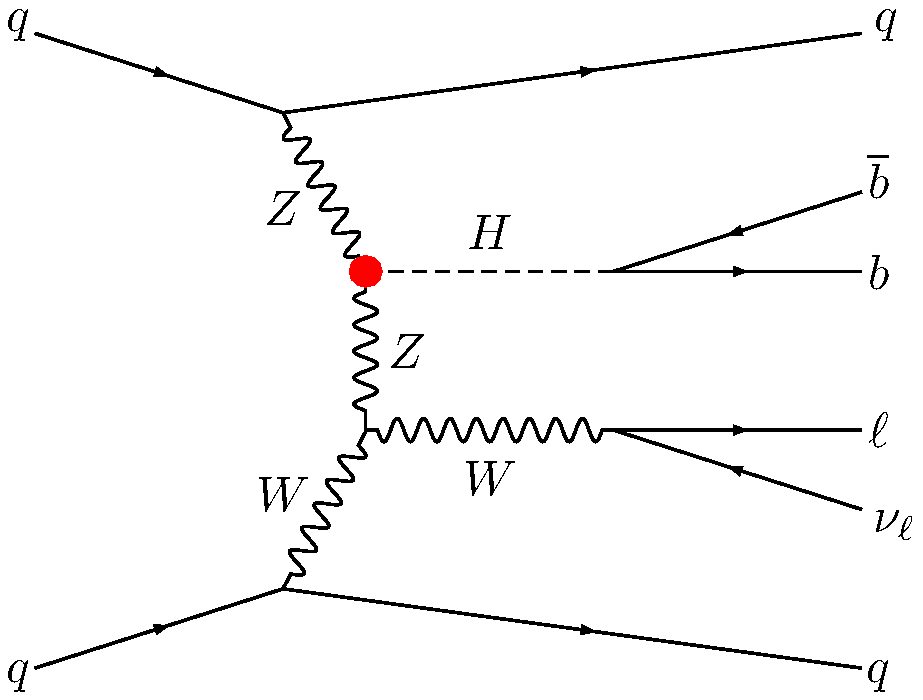
\includegraphics[width=0.3\textwidth]{fig/feynman/vbswh/vbswh_1.pdf}}\quad
    \subfloat{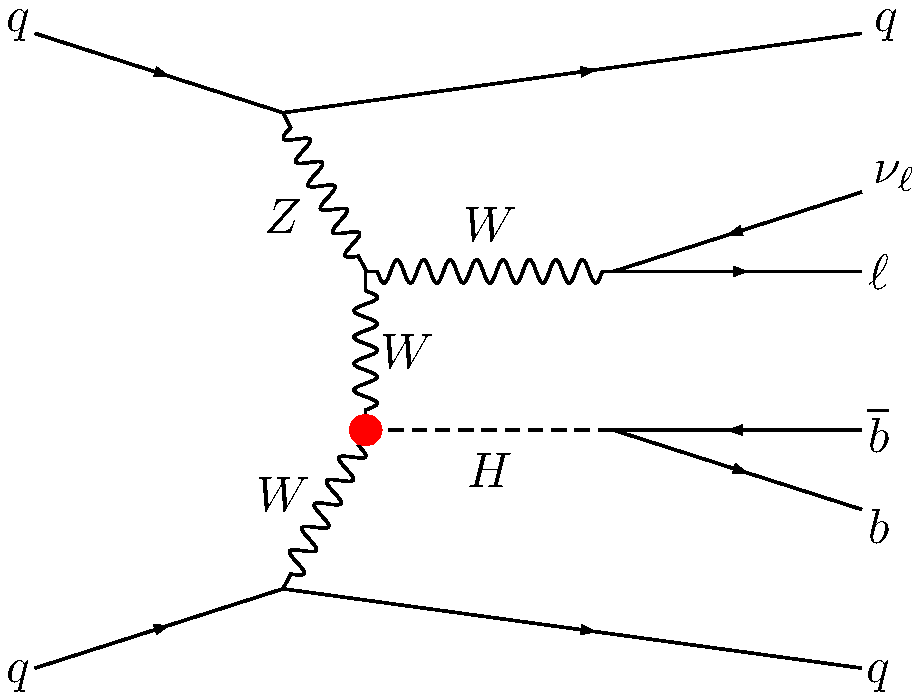
\includegraphics[width=0.3\textwidth]{fig/feynman/vbswh/vbswh_2.pdf}}\quad
    \subfloat{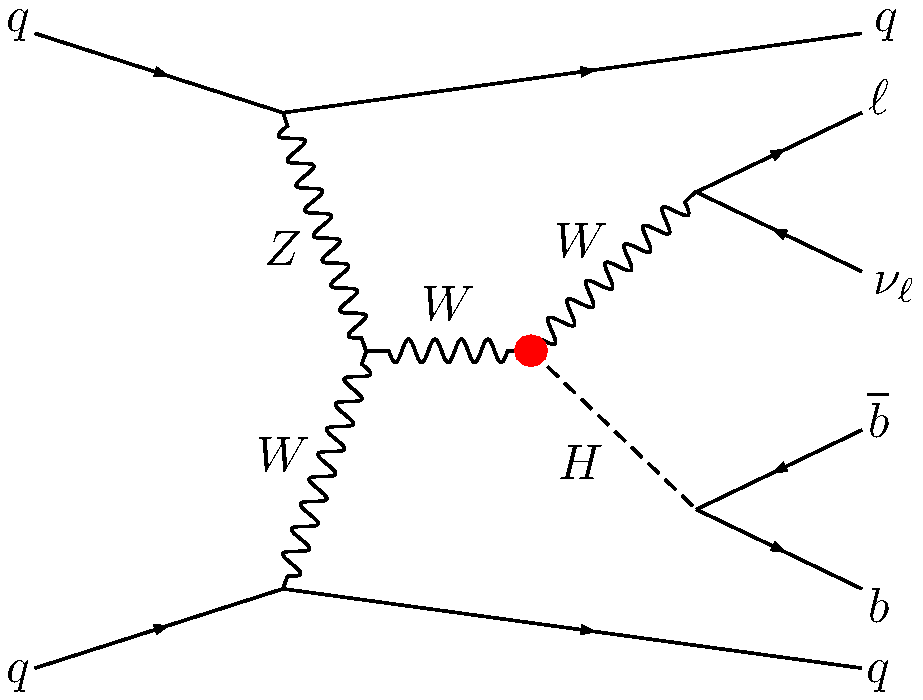
\includegraphics[width=0.3\textwidth]{fig/feynman/vbswh/vbswh_3.pdf}}
    \caption{
        Leading-order Feynman diagrams for VBS production of a W and Higgs boson, where the W decays leptonically and the Higgs decays to b quarks. 
        The Higgs coupling to W bosons \kW and Z bosons \kZ is denoted by a red circle (\textcolor{red}{\ding{108}}). 
    }
    \label{fig:vbswh_feynman}
\end{figure}

A specific final state is intentionally selected for its uniqueness---making it easier to find amidst the haystack. 
First, leptons are preferred in the final state over jets, due to the sheer size of the ``QCD'' background, the most populous physics process produced at the LHC. 
Then, $\PW\to\ell\nu$ is preferred over $\PZ\to\ell\ell$, since there are fewer backgrounds with only one lepton in the final state. 
Finally, $\PH\to\PQb\PAQb$ has the largest branching ratio, and it can be identified using the latest advances in artificial intelligence. 
Only a few background processes can produce such a final state and modifications to \lambdaWZ would greatly increase the energy of the final state particles, while also increasing the overall cross section. 

\section{The backgrounds}
The main background process for this analysis comes from \ttbar production, wherein a top and antitop quark are produced. 
The two quarks decay to a bottom quark and W boson. 
Primarly, this background looks most like signal when one of the W bosons decays leptonically. 
\begin{figure}[htb]
    \centering
    \subfloat[$\ttbar + \text{jet}$]{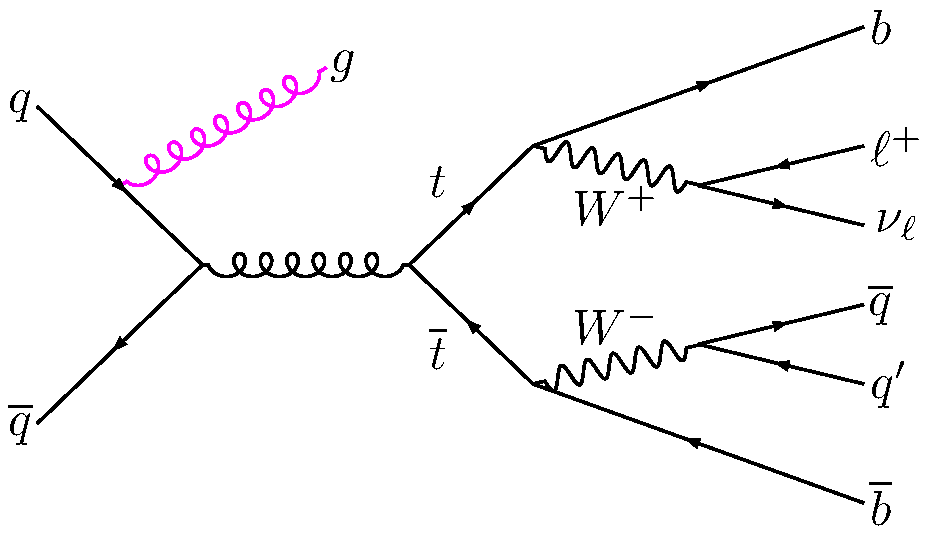
\includegraphics[width=0.4\textwidth]{fig/feynman/ttbar/ttbar_onelep_extraJet.pdf}\label{fig:ttbar1l}}\quad
    \subfloat[$\ttbar + \PV$]{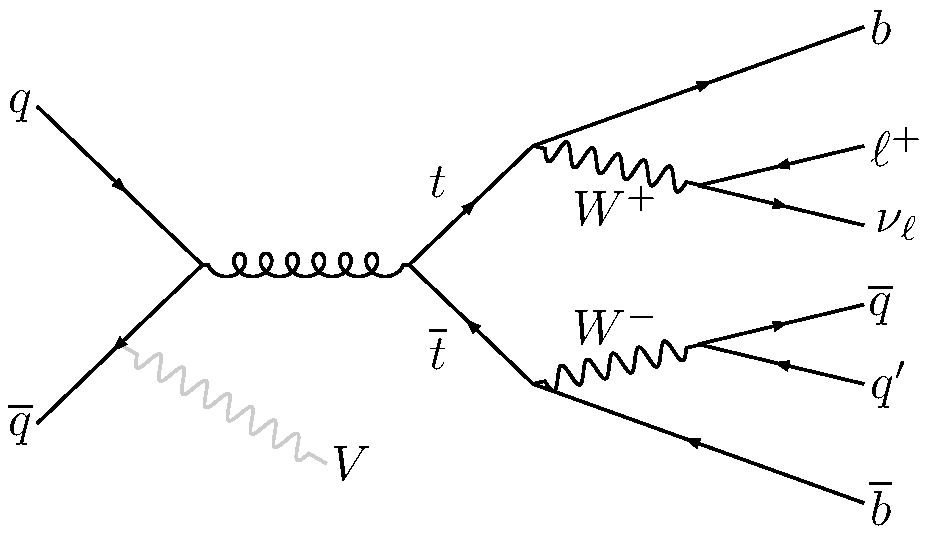
\includegraphics[width=0.4\textwidth]{fig/feynman/ttbar/ttV_onelep.pdf}\label{fig:ttV1l}}
    \caption{
        Feynman diagram for \ttbar production in the single-lepton final state with (a) an extra jet from a gluon or (b) an extra vector boson ($\PV = \PW$ or \PZ) radiated from one of the incoming partons.  
    }
    \label{fig:ttbar}
\end{figure}

\section{Event selection}

\section{Background estimation}

\section{Results}
\begin{figure}[htb]
    \centering
    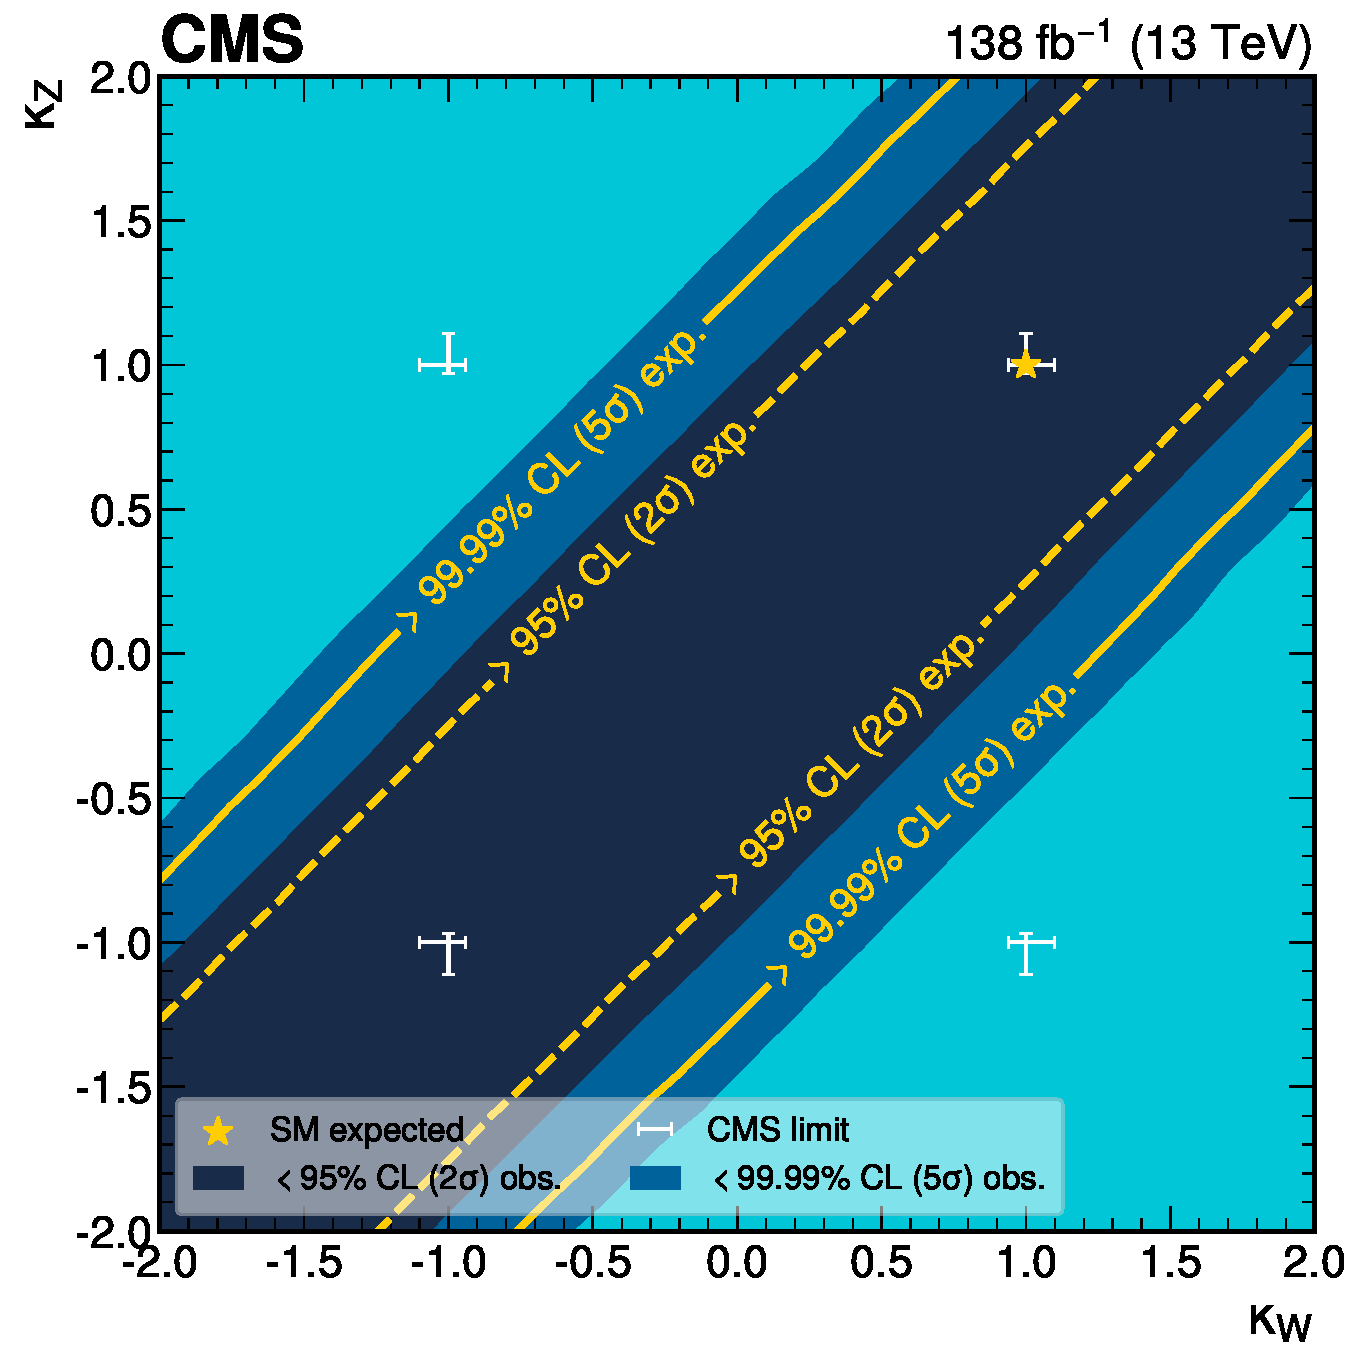
\includegraphics[width=0.5\textwidth]{fig/vbswh/exclusion_2D_contours_unblinded.pdf}
    \caption{
        Exclusion significance plotted as a function of \kW and \kZ.
        Opposite-sign scenarios ($\lambdaWZ < 0$) are excluded well beyond 5$\,\sigma$. 
    }
    \label{fig:vbswh_limit}
\end{figure}
